\chapter{Versuchsdurchführung}
    \section{Aufnahme der Eingangskennlinie}
        Für die Aufnahme der Eingangskennlinie haben wir die Schaltung ~\ref{fig:npn_transistor} auf der Seite ~\pageref{fig:npn_transistor} etwas vereinfacht. Die folgende Abbildung zeigt wie für die erste Messung die Schaltung in LTSpice ausgesehen hat. 

        \begin{figure}[h!]
            \centering
           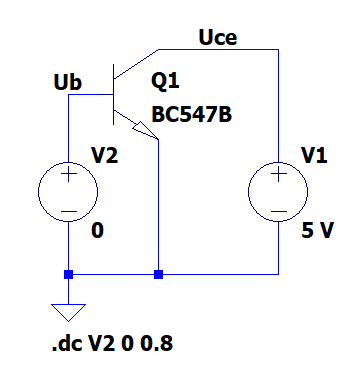
\includegraphics[width=5cm]{Bilder/eingangskennlinieSchaltung.png}
           \caption{Schaltung zur Aufnahme der Eingangskennlinie eines NPN-Transistor Type BC547B}
           ~\label{fig:eingangskennlinieSchaltung}
        \end{figure}
        
        Bei der Messung des Stroms \(I_B\) kamen folgende Werte zusammen. 

        \begin{figure}[h!]
            \centering
           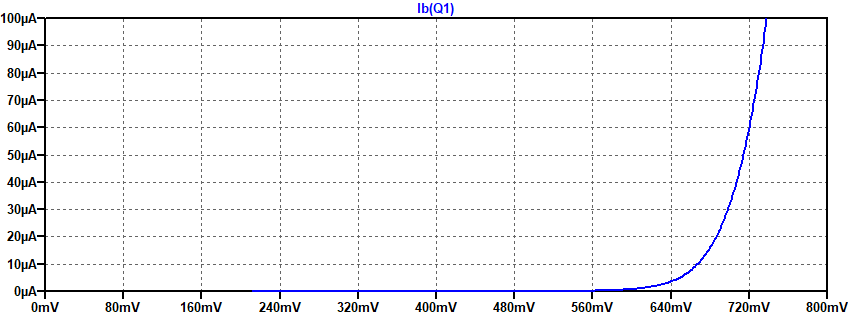
\includegraphics[width=15cm]{Bilder/eingangskennlinie.png}
           \caption{Messwerte der Eingangskennlinie eines NPN-Transistor Type BC547B}
           ~\label{fig:eingangskennlinie}
        \end{figure}